\documentclass[12pt, 
    twoside=false, 
    bibliography=totoc, 
    numbers=endperiod, 
    headings=normal, 
    toc=chapterentrydotfill
    ]{scrbook}
\usepackage[T1]{fontenc}
\usepackage[utf8]{inputenc}
\usepackage[ngerman]{babel}
\usepackage{blindtext}
\usepackage{csquotes}
\usepackage{booktabs}
\usepackage{array}
\usepackage{setspace}
\usepackage{mathpazo}
\usepackage{graphicx}
\usepackage{etoolbox}
\usepackage[
  	pdfstartview=FitH,   
  	pdffitwindow=true,
  	colorlinks,
  	linkcolor=black,
  	anchorcolor=black,
  	citecolor=black,
  	urlcolor=black
  	]{hyperref}
\usepackage[labelfont=bf]{caption}
\usepackage{float}
\usepackage[
    backend=biber, 
    style=authoryear-ibid, 
    eprint=false,
    url=false,
    doi=false,
    isbn=false,
    dashed=false
    ]{biblatex}
\addbibresource{Bib.bib}

% Layoutanpassungen
\setkomafont{sectioning}{\normalcolor\bfseries}
\renewcommand*{\chapterheadstartvskip}{\vspace*{-\topskip}}
\KOMAoptions{headsepline = true}
\setlength{\textheight}{1.05\textheight}
\AtBeginEnvironment{quote}{\singlespacing\small}

\begin{document}

\begin{titlepage}
    \begin{minipage}[t]{0.6\textwidth}
    \flushleft 
    Universität Hamburg \\
    Fachbereich: Sozialwissenschaften \\
    Fachgebiet: Politikwissenschaft \\
    Seminar: Forschungsseminar Vergleichende und Regionalstudien \\ 
    Dozenten: Prof. Kai-Uwe Schnapp \\
    PD Dr. Falk Daviter \\
    Wintersemester 2018/19 \\
    \end{minipage}
    \hfill
    \begin{minipage}[t][1.7cm][b]{0.35\textwidth}
    
\includegraphics[width=\textwidth]{images/UHH-Logo_2010_Farbe_CMYK.pdf}
    \end{minipage}
    
    \vspace*{\fill}
    \begin{center}
	\vspace{1cm}\noindent {\textbf{Projektarbeit}} \vspace{0.2cm} \\
	\textbf{\Large Geschlechtsbezogene Repräsentationsunterschiede in Parlamentsdebatten \\
	\vspace {0,5cm} \small\emph{Inwiefern unterscheiden sich Redebeiträge und Verhalten von weiblichen und männlichen Abgeordneten im 19. Deutschen Bundestag bezüglich Häufigkeit, Thematik und Geschlechterneutralität}} \\
	\vspace{0.5cm}
	30.03.2019
	\end{center}
    \vspace*{\fill}
	
	\begin{minipage}[t]{0.48\textwidth}
    \flushleft 
    Gina-Gabriela Görner \\
    Matrikelnummer: 6436971 \\
    Friedensallee 15 \vspace{0.1cm} \\ 
	22765 Hamburg \vspace{0.1cm}  \\
	E-Mail: Gina-Gabriela.Goerner@Uni-Hamburg.de \\ 
    \end{minipage}
    \begin{minipage}[t]{0.48\textwidth}
	\flushleft
	Josef Holnburger \\
	Matrikelnummer: 6524900 \\
	Beuthstraße 1 \vspace{0.1cm} \\
	10117 Berlin \vspace{0.1cm} \\
	E-Mail: josef@holnburger.com \\
    \end{minipage}

\end{titlepage}

\frontmatter

\tableofcontents

\listoffigures
\addcontentsline{toc}{chapter}{\listfigurename} !!!hier nur ein i im Inhaltsverzeichnis !!!
\vspace*{24pt}
{\let\clearpage\relax \listoftables}	
\addcontentsline{toc}{chapter}{\listtablename}

\mainmatter

\setstretch{1.5}


\chapter{Einleitung}\label{Einleitung} 

\begin{quote}
    \enquote{ Gender equality in political representation may be described within both optimistic and pessimistic stories.} \parencite[149]{celis_2018}
\end{quote}


Die machtpolitische Gleichstellung der Geschlechter sowie die politische Ressourcenverteilung in den industrialisierten Demokratien ist in den letzten fünfzig Jahren enorm gewachsen \parencite[318]{coffe_2010}. Es gibt mehr weibliche Parlamentarierinnen (aus dem englischen \emph{Members of Parliament} = MPs) als je zuvor und eine Rekordzahl von Frauen nimmt Führungspositionen in den Nationalen Regierungen \parencites{lovenduski_2005}{paxton_2007}, mit vielen wichtigen Konsequenzen für politische Ergebnisse und Prioritäten \parencites{bolzendahl_2007}{carroll_2001}{waring_2000}[318]{coffe_2010}, ein. Dennoch sind derzeit weniger als ein Viertel Frauen (24,3 Prozent) in den weltweiten Parlamenten vertreten \parencite{ipu_2019}. Repräsentative Institutionen werden trotz eines langen Kampfes um Gleichstellung noch immer von Männern dominiert \parencites[149]{celis_2018}[497 f.;]{childs_2013}{dahlerup_2013} {bjarnegard_2013} und es ist nicht umstritten zu behaupten, dass die Gleichstellung der Geschlechter nicht erreicht wurde \parencite[150]{celis_2018}. Eine Gleichstellung wird hierbei nicht nur über die Anzahl der Sitze in repräsentativen Parlamenten bestimmt, sondern ergibt sich durch eine Vielzahl an Faktoren, u.a. auch der sprachlichen Einbeziehung beider Geschlechter (*aller Geschlechter - Hinweis iwo anbringen!!!) in den Parlamentsdebatten und dem Nichtvorhandensein von geschlechterspezifischem Verhalten sowie einer geschlechterunspezifischen Themenwahl. Da die Gleichstellung und Repräsentation von Frauen in Parlamenten in Form der Anzahl an Sitzen im Parlament in einer Vielzahl an Erhebungen bereits untersucht wurde (QUELLLEN!!!!!), sind letztere Faktoren Untersuchungsgegenstand der vorliegenden Arbeit. 

\begin{quote}
     \enquote{Gender equal representation is not only about the proportion of men and women legislators or the outcomes of politics}\parencite[197]{erikson_2018}
 \end{quote}

In Anlehnung an \textcite{erikson_2018} wird eine geschlechtergerechte Repräsentation in der vorliegenden Arbeit weder daran gemessen, ob eine gleiche Anzahl an Frauen und Männern im Parlament vertreten ist, noch anhand der politischen Ergebnisse. Ausgangspunkt dieser Arbeit für eine \emph{geschlechtergerechtere Repräsentation} ist ein mehrdimensionaler Repräsentationsbegriff:

Repräsentation gilt als ein Kernkonzept in der Erforschung und Praxis der Politik und kann in verschiedenen, miteinander verbundenen Dimensionen betrachtet werden. Es kann hierbei zwischen dem, was repräsentiert wird, wie es repräsentiert wird und wer repräsentiert, unterschieden werden \parencite[557]{galligan_2007}. In den meisten Fällen bieten sowohl die Wähler*innen, Parteien, Wahlen und Gesetzgeber*innen den Hintergrund für eine Diskussion über eine oder mehrere Elemente der jeweiligen Repräsentationsdimension \parencite[557]{galligan_2007}.
In der vorliegenden Arbeit werden fünf Repräsentations-Dimensionen definiert und differenziert voneinander betrachtet. Obwohl keine der im Folgenden genannten Dimension gänzlich unabhängig von den anderen Dimensionen analysiert werden kann, werden sie in dieser Arbeit zunächst klar voneinander getrennt um die Komplexität der verschiedenen Dimensionen zu reduzieren. Eine Hierarchisierung der Dimensionen ist kein Bestandteil dieser Analyse. Das Ziel liegt in einer differenziert gewichteten Analyse der folgenden fünf Repräsentationsebenen:

\begin{itemize}
    \item Ebene A: Weibliche Repräsentation im Parlament: Sind Frauen im Parlament vertreten? Wie viele Frauen sind relativ und absolut im Parlament vertreten? 
    \item Ebene B: Weibliche Repräsentation bei den Parlaments-Debatten: Nehmen Frauen an den Parlaments-Debatten teil? Nehmen Frauen relativ und absolut gleich viel an den Parlaments-Debatten teil? 
    \item Ebene C: Repräsentation von Frauen in den Parlaments-Debatten: Werden in den Parlaments-Debatten Frauen ebenso wie Männer sprachlich repräsentiert? Wird Gender-Fair-Language (GFL) genutzt? Wird GFL von weiblichen und männlichen MPs in gleichem Maße genutzt? 
    \item Ebene D: Repräsentation von geschlechtsbezogenen Stereotypisierungen: Werden gesellschaftliche geschlechtsbezogene Stereotypisierungen reproduziert? Unterscheidet sich die Thematisierung in den Reden von Frauen und Männern? 
    \item Ebene E: Repräsentation von geschlechtsspezifischen Verhaltensmustern: Werden in den Parlaments-Debatten frauenfeindliche Verhaltensmuster reproduziert? Werden Frauen häufiger negativ unterbrochen?  
\end{itemize}

In der abschließenden !!!Diskussion/ (oder) in Kapitel ?? wird!!! ausführlich auf eine mögliche Vernetzung der einzelnen Dimensionen eingegangen, sodass diese 5 Dimensionen zunächst gesondert voneinander betrachtet und analysiert werden können.  !!! Hinweis: Diese Dimensionen sind mir jetzt neu, und ich weiß noch nicht, wieso sie als Ebenen definiert werden. Hier brauchen wir noch fundierten Hintergrund. Muss erst Ebene 1 erreicht werden, um Ebene 2 zu erfüllen? Welche Hintergrund hat diese Argumentaiton? !!!


\chapter{Theoretischer Hintergrund}

\section{Workplace-Approach: Politik als Arbeitsperspektive} 

Die bisherige Forschung zur politischen Repräsentation von Frauen fokussiert primär deskriptiven Themen, wie etwa die Frage danach, wie gesetzgebende Gremien durch Quoten geschlechtsgerechter strukturiert werden können \parencites [vgl.]{dahlerup_2005}{schwindt-bayer_2009} oder substantive Themen, welche beispielsweise untersuchen, ob weibliche Gesetzgeberinnen einen positiven Einfluss auf genderfreundliche politische Ergebnisse haben \parencites [199]{erikson_2018}{beckwith_2007}. Den inneren Mechanismen der gesetzgebenden Körperschaften sowie der Frage, \enquote{how the political game itself is gendered} wurde bisher weniger empirische Aufmerksamkeit gewidmet \parencites[199]{erikson_2018}[vgl.][]{childs_2016}{dahlerup_2013}{wangnerud_2015}.

Ein Ausgangspunkt der vorliegenden Arbeit ist, dass das legislative Arbeitsumfeld für sich genommen ebenso wichtig ist, wie die Möglichkeiten der weiblichen Gesetzgeberinnen, die Ergebnisse zu beeinflussen. Politikerinnen sollten in der Lage sein, ihre Aufgaben als Gesetzgeberinnen auf Augenhöhe mit ihren männlichen Kollegen zu erfüllen \parencite[199]{erikson_2018}. 

\textcites{dahlerup_2006}{dahlerup_1988} !!!HIER WICHTIG; DAHLERUP LESEN ALS PRIMÄR und wie formatieren?) unterscheidet zwischen zwei verschiedenen Perspektiven der substantiellen Repräsentation von Frauen. Zum Einen existiert die politische \emph{Outcome-Perspektive}, welche die wissenschaftliche Literatur zur substantiellen Repräsentation von Frauen tendenziell dominiert. Zum Anderen existiert die Perspektive der Politik als \emph{Arbeitsperspektive}, welche bisher weniger häufig diskutiert wurde \parencites[513]{dahlerup_2006}[199]{erikson_2018}. 

Während sich die Outcome-Perspektive darauf konzentriert, ob weibliche Gesetzgeberinnen den Inhalt politischer Entscheidungen beeinflussen, indem sie diese geschlechtsfreundlicher gestalten oder eine feministische Agenda verfolgen, beschäftigt sich die zweite Perspektive mit den Möglichkeiten, wie weibliche MPs als Repräsentantinnen gleichberechtigt mit ihren männlichen Kollegen auftreten können \parencites[199]{erikson_2018}{dahlerup_2006}{dahlerup_1988}.

Der in dieser Arbeit verwendete \emph{‚workplace approach‘} oder die bereits genannte Arbeitsperspektive zielt in Anlehnung an \textcite{erikson_2018} insgesamt darauf ab, die Repräsentation von Frauen aus einer breiteren Perspektive zu betrachten, indem der Fokus von den Ergebnissen auf die geschlechtsspezifischen Bedingungen innerhalb der Legislative verlagert wird. Mit Orientierung an die Arbeiten von \textcites{dahlerup_2006}{dahlerup_1988}{erikson_2018} werden die  Arbeitsbedingungen im deutschen Bundestag in der vorliegenden Arbeit als wichtig sowie als wesentlicher Bestandteil der Möglichkeiten, wie Frauen die politischen Ergebnisse beeinflussen können, eingestuft. Die sprachliche Einbeziehung von Frauen innerhalb der Parlamentsdebatten zählt hierbei ebenso wie geschlechterneutrales Verhalten zu den Arbeitsbedingungen im Deutschen Bundestag. (hier noch eine Überleitung? oä.? ....!!!!)

\section{Legislative Gremien als maskuline Organisation }

Innerhalb der legislativen Gremien wurde das Geschlechterregime ebenso wie in anderen von Männern dominierten Sektoren häufig als ‚permeated by a culture of masculinity‘ beschrieben \parencites[200]{erikson_2018}{lovenduski_2005}. In Anlehnung an \textcite{acker_1990} zeigt sich dies beispielsweise in der Existenz von formalen Regeln, die von Männern geschaffen wurden und einer männlich dominierten Organisation angepasst sind, sowie in Normen, wie sich ein (männlicher) Politiker präsentieren und verhalten soll \parencites[200]{erikson_2018}[48]{acker_1990}. Frauen werden infolgedessen mit dieser bereits existierenden ‚culture of masculinity‘ konfrontiert, die als institutionelle Einschränkung fungieren kann wenn beispielsweise ihre Arbeit dadurch behindert wird \parencites[200]{erikson_2018}[47-56]{lovenduski_2005}. \textcite{erikson_2018} verweisen auf sozialpsychologische Forschungen, wonach Frauen in männerdominierten Bereichen häufig diskriminiert werden weil es an Übereinstimmungen zwischen den männerdominierten beruflichen Normen und den Eigenschaften mit denen Frauen typischerweise assoziiert werden mangelt \parencites[vgl.][]{burgess_1999}{eagly_2002}{heilman_2001}{heilman_2004} noch nicht geprüft !!!))). Frauen riskieren Diskriminierungen, weil sie entweder als weniger kompetent angesehen werden oder weil sie weibliche Attribute verletzen, wenn sie sich den Normen anpassen \parencite[200]{erikson_2018}. Die Folgen sind neben der Disqualifikation, die Abwertung der Leistungen sowie die ungleiche Behandlung von Frauen bishin zu Belästigungen \parencites[200]{erikson_2018}{heilman_2001}{burgess_1999}:

\begin{quote}
     \endquote{The gendered consequences of masculine norms are often manifested in the first case in the disqualification of women or the devaluation of their performance, whereas they often take the form of a disparate treatment of women in the second, including harassment}\parencite[200]{erikson_2018}
\end{quote}

Informelle Praktiken und Normen innerhalb des Arbeitsumfeldes können als Hindernisse für die Schaffung eines geschlechtergerechten Arbeitsumfeldes angesehen werden \parencite[200]{erikson_2018}. Ausgangspunkt der vorliegenden Arbeit ist die Annahme, dass der 19. Deutschen Bundestag von einer 'culture of masculinity' durchzogen ist und u.a. dadurch die Geschlechtergerechtigkeit des Arbeitsumfeldes zum Nachteil von Frauen beeinflusst wird. (!!!oder?!!!)

\chapter{Relevanz des Forschungsgegenstandes}

In demokratischen Systemen sind Parlamentarier*innen nicht nur wichtige Akteure als Gesetzgeber*innen, sondern auch als Teilnehmer*innen an der öffentlichen Debatte und als Mitwirkende an der öffentlichen Meinungsbildung \parencite[188]{dahlerup_2018}.
In Anlehnung an \textcite{back_2018} gibt es mehrere Gründe, warum die Auswirkungen des Geschlechts auf das Verhalten der legislativen Debatte interessant sind. Ein wichtiger Grund ist hierbei die zentrale Rolle der legislativen Debatte in parlamentarischen Demokratien. Die Gesetzte werden in der Regel von Abgeordneten diskutiert bevor sie darüber abstimmen \parencites[2]{back_2018}{back_2016}{proksch_2015}. 
Die Debatten können in Anlehnung an \textcite[1]{proksch_2015} ebenso als Foren für öffentliche Kommunikation angesehen werden, welche von den Parteien und ihren Abgeordneten für Wahlzwecke genutzt werden \parencite[2]{back_2018}. Ausgehend davon, dass Debatten Auswirkungen auf die Politikgestaltung haben und von Parteien genutzt werden, um die Medien und die Wähler*innen zu informieren und zu beeinflussen, ist es von Relevanz ob dabei ein Geschlecht unterrepräsentiert ist \parencite[2]{back_2018}. Welche Auswirkungen eine Unterrepräsentation von Frauen für politische Entscheidungen haben kann, wird in KAPITEL??? erläutert. \textcite{back_2018} argumentieren, dass selbst ohne signifikanten Einfluss der Debatte auf politische Ergebnisse, die geschlechtsspezifischen Sprachmuster zu einer geringeren Legitimität des demokratischen Systems führen können \parencite[2]{back_2018}.
Die Relevanz von Geschlechtergleichheit auf politischer Ebene kann nicht (mehr) in Frage gestellt werden. Dennoch gibt es Uneinigkeit darüber, ob und inwiefern eine Geschlechtergleichheit bereits erreicht wurde und auf welchen Ebenen eine Gleichstellung der Geschlechter bereits abgeschlossen oder nahezu umgesetzt wurde.

\begin{quote}
    \enquote{ Gender equality in political representation may be described within both optimistic and pessimistic stories.} \parencite[149]{celis_2018}
\end{quote}

In Anbetracht des Zitates von \textcite{celis_2018} und einer zunehmenden deskriptiven Repräsentation von Frauen in den Parlamenten ist es essentiell, eine Analyse nicht ausschließlich aus dieser Ebene der Repräsentation durchzuführen und sich optimistisch mit einer Zunahme an Frauen in den Parlamenten zufrieden zu geben, sondern die Forderung nach Geschlechtergerechtigkeit, auch im Sinne gleicher und gleichwertiger Repräsentation auf allen fünf Ebenen zu fordern und fördern. 

\begin{quote}
    \enquote{While women have made substantive progress in their representation in politics, they are still well underrepresented in political life in most nations} \parencite[2]{coffe_2013}
\end{quote}

Wenngleich ein politischer Konsens darin besteht, dass Gleichheit und Gerechtigkeit, sowie implizit Geschlechtergleichheit und ,-gerechtigkeit eine fundamentale Komponente von Demokratie darstellt, gibt es noch immer einen weltweiten Gender-Gap in den Parlamenten (ausgenommen ist hierbei..!!!)weltweit jedem Parlament (NOCH MAL PRÜFEN - ob Ruanda).  

!!!
]]]]]]
 Repräsentation von Frauen für Demokratie notwendig .... . EINLEITEN/ÜBERLEITEN... ???? ........Überleitung??????!!!
 


Anne Phillips gilt als eine der wichtigsten Vertreterinnen auf dem Gebiet der parlamentarischen Repräsentativität von Frauen. In ihrem Werk \emph{politics of presence} \parencite*{phillips_1998} analyisiert Phillips unter anderem die Bereitschaft von Frauen, als Parlamentskandidatin ausgewählt zu werden, Ministerin zu werden und Wahlen zu gewinnen \parencite[vgl.][416f.]{blaxill_2016}. Frauen sammeln im täglichen Leben andere Erfahrungen als Männer. Hierbei bezieht sich \textcite{phillips_1998} unter anderem auf die Kindererziehung, Bildung, Auswahl an Berufen, Unterscheidung von bezahlter und unbezahlter Arbeit sowie auf Gewalterfahrungen und sexuellen Belästigungen. \textcite{phillips_1998} plädiert aufgrund der unterschiedlichen Lebenserfahrungen für die notwendige Repräsentation von Frauen im Parlament, um andere Frauen vertreten zu können \parencite[vgl.][52]{wangnerud_2009}.

\begin{quote}
    \enquote{There are particular needs, interests, and concerns that arise from women's experience, and these will be inadequately addressed in a politics that is dominated by men. Equal rights to a vote have not proved strong enough to deal with this problem; there must also be equality among those elected to once} \parencite[66]{phillips_1998}
\end{quote}

Bereits Piktin \parencite*{pitkin_1972} argumentierte in ihrem Hauptwerk "The Concept of Representation", dass der Interessenbegriff in der Repräsentationsdebatte omnipräsent ("ubiquitious") ist \parencite[69]{wangnerud_2000}. Für Pitkin sind es die Parlamentarier\emph{innen}, welche sich den Wünschen und Interessen, dem Wohlergehen sowie Themen der Frauen widmen und diese vertreten \parencites[vgl.][413]{blaxill_2016}{pitkin_1972}. In Anlehnung an Phillips' Theorie der \emph{politics of presence} \parencite*{phillips_1998} wird angenommen, dass weibliche Politikerinnen die Interessen und Wünsche weiblicher Bürgerinnen besser als männliche Politiker repräsentieren können. Hierbei wird die deskriptive mit der substantiellen Repräsentation verknüpft \parencite[52]{wangnerud_2009}: ein höherer Frauenanteil in Parlamenten führt zu einer stärkeren Thematisierung der Belange von Frauen.

Während die Forderungen einer deskriptiven parlamentarischen Geschlechtergleichheit ebenso wie die Forderungen nach substantieller Geschlechtergleichheit bereits ihre Wege in die wissenschaftliche Diskussion und in die Politik gefunden haben, wurde der geschlechtergerechten Sprache sowie dem geschlechtsbezogenen Verhalten in den Parlamenten bisher weniger Aufmerksamkeit gewidmet. 
Laut \textcite{menegatti_2017} ist die Sprache eine der einflussreichsten Faktoren, wodurch Sexismus und Geschlechterdiskriminierung gefördert und reproduziert werden \parencite*[1]{menegatti_2017}. Sprache kann hierbei insbesondere die sozialen Asymmetrien von Status und Macht zugunsten des Mannes reproduzieren \parencite[1]{menegatti_2017}. Es existier[t]en einvernehmliche Normen, wonach der prototypische Mensch ein Mann ist, was sich in den Strukturen vieler Sprachen widerspiegelt und darin verankert ist. Viele grammatikalische und syntaktische Regeln sind so aufgebaut, dass weibliche Ausdrücke normalerweise von entsprechenden männlichen Formen abgeleitet werden \parencite*[1]{menegatti_2017}. Männliche Substantive und Pronomen werden beispielsweise häufig mit einer generischen Funktion verwendet um sich sowohl auf Männer als auch auf Frauen zu beziehen. Auf diese Weise verschwinden Frauen aus der mentalen Repräsentationen \parencites{vaughan_2018}{stahlberg_2001}. Maskuline Generika lassen Leser*innen und Hörer*innen mehr in männlichen als weiblichen Personenkategorien denken \parencites[2]{sczesny_2016}{stahlberg_2007}.

\begin{quote}
    \enquote{Given that language not only reflects stereotypical beliefs but also affects recipients’ cognition and behavior, the use of expressions consistent with gender stereotypes contributes to transmit and reinforce such belief system and can produce actual discrimination against women} \parencite[2]{menegatti_2017}
\end{quote}

\begin{itemize}
    \item - gendered -shelley et al ? (ich konnte dem Text nicht sehr viel entnehmen!) 
    \item - Fehlt hier noch - Stereotypen als Theoretischer Unterbau und Unterbrechungen ...
\end{itemize}



\section {Derzeitiger Forschungsstand und relevante Studien }

\subsection{Frauen im Parlament}

In der Forschung zu Frauen im Parlament wird generell zwischen einer deskriptiven, substantiellen und (in einigen Fällen) der symbolische Form der Repräsentation unterschieden. Bei der substantiellen Repräsentation von Frauen handelt es sich um ein bisher weniger wissenschaftlich erforschtes Feld als die Analyse der deskriptiven Repräsentation \parencite[59]{wangnerud_2009}. 
Letzteres legt den Schwerpunkt auf die Analyse der Anzahl von Frauen in repräsentativen Institutionen, ersteres untersucht hingegen die Auswirkung der Präsenz von Frauen in Parlamenten \parencites[14]{coffe_2013}[52]{wangnerud_2009}.
Die zentralen Fragen lauten hierbei:

\begin{quote}
  \enquote{[W]hether the widely professed aspiration to feminise democracy -- and in so doing to politically empower women -- is a matter largely of symbolism or substance […]}
  \enquote{[…] wheter the priority should simply be to increase the proportion of women MPs in Parliament […] or as Hanna Pitkin argued in 1967, to represent minds as well as bodies.}
  \parencite[413]{blaxill_2016}
\end{quote}

%
Die Theorie der \emph{politics of presence} \parencite{phillips_1998} diente Wängnerud \parencite*{wangnerud_2000} als Ausgangspunkt für ihre Forschung im Schwedischen Parlament (\enquote{Testing the Politics of Presence, Women's Representation in the Swedish Riksdag}, 2000). Wägnerud prüft hierbei die Hypothese, ob weibliche Politikerinnen die Interessen von Frauen stärker vertreten als männliche Politiker \parencite[84]{wangnerud_2000} und kommt zu folgendem Ergebnis: \enquote{[It is] difficult to repudiate the conclusion that women's interes are primarily represented by female politicians} \parencite[][84]{wangnerud_2000}. Laut Wängnerud \parencite*{wangnerud_2000} bleibt es jedoch ausstehend welche Auswirkungen zu erwarten sind, wenn die Zahl der Frauen im Parlament steigt \parencite{wangnerud_2009}.
Die Forschung von \textcite{celis_2008} greift diese Annahme empirisch auf und untersucht, in welchem Ausmaß die Bedürfnisse und Interessen von Frauen gesteigert werden, wenn die Anzahl von Frauen in politischen Entscheidungen zunimmt \parencite[vgl. auch][4]{galligan_2016}. Ein einfacher Anstieg der Anzahl von Frauen reicht nach \textcite{celis_2008} nicht aus, um einen signifikanten Einfluss zu erreichen. In Anlehnung an Caul \parencite*{caul_2001} sei es beispielsweise notwendig, dass weibliche Abgeordnete in einflussreichen, wichtigen Positionen vertreten sind, um substantielle Repräsentation zu ermöglichen \parencites{caul_2001}[vgl. auch][14]{coffe_2013}.
Auch die Forschung von \textcite{back_2014} fragt nach den Auswirkungen, wenn die Zahl der Frauen im Parlament steigt und kommt zu folgendem Ergebnis: 

\begin{quote}
  \enquote{The variation found here is, however, not in line with the hypothesis suggesting that increased descriptive representation should lead to a rise in the substantive representation so that the prediction drawn from the critical mass theory is not given support here. Instead, we find that women are more underrepresented in legislative debates when they represent parties with many female MPs.}
  \parencite[17]{back_2018}
\end{quote}
besser: nicht das Kapitel critical mass aufmachen, oder?????? 
\begin{quote}
  \enquote{The variation found here is, however, not in line with the hypothesis suggesting that increased descriptive representation should lead to a rise in the substantive representation [...]is not given support here. Instead, we find that women are more underrepresented in legislative debates when they represent parties with many female MPs.}
  \parencite[17]{back_2018}
\end{quote}


\textcite{back_2018} haben eine vergleichende Analyse der Auswirkungen des Geschlechts der Abgeordneten auf ihre Gesetzgebungstätigkeit durchgeführt. Im Vordergrund steht hierbei die Frage, ob weibliche Vertreterinnen weniger an Gesetzgebungsdebatten teilnehmen und ob das im Parlament diskutierte Thema für ihre Beteiligung von Bedeutung ist. \textcite{back_2018} untersuchen hierfür länderübergreifend sieben europäische Länder bezüglich der Themen und Redeanteile weiblicher Abgeordneter und resümieren, dass Frauen in Parlamenten seltener das Wort ergreifen. Dieses Ergebnis ist nicht auf einen generell niedrigeren Anteil an Frauen in den Parlamenten zurückzuführen, so \textcite{back_2018}. Frauen in Parteien mit einem geringen Frauenanteil ergreifen laut der Untersuchung von \textcite{back_2018} sogar häufiger das Wort als Frauen in Fraktionen mit einem hohen Anteil an weiblichen Mitgliedern \parencite*[17]{back_2018}. 

Aus den Untersuchungen von \textcite{kathlene_1994} zu US-Staatsgesetzten und \textcite{back_2014} zum schwedischen Riksdag geht hervor, dass Frauen in Debatten seltener sprechen, während andere Fallstudien von \textcite{noch eingeben}Broughton und Palmieri (1999, zu Australien),\textcite{noch eingeben} Murray (2010, zu Frankreich) und Wang\textcite{noch eingeben} (2014, zu Uganda) zeigen, dass „‘women are equally active debate participants as their male colleagues’ \parencites[254]{taylor-robinson_2014}[2]{back_2018}. In Anlehnung an \textcite{back_2018} kann davon ausgegangen werden, dass es eine länderübergreifende Variation der Rolle des Geschlechts in Debatten gibt\parencite[2]{back_2018}. Eine gesonderte Untersuchung der Rolle des Geschlechts in den Debatten des Deutschen Bundestags erscheint auch aus dieser Perspektive notwendig. 
[[[[[Das könnte im weiteren verlauf vll eine gute Verbindung sein, aber noch zu prüfen::!!! Taylor-Robinson (2014) looks at debate participation as one type of substantive representation and refers to a seminal study of US state legislatures which shows that women speak less frequently in debates \parencite{kathlene_1994}.]]]]


In einer früheren Studie konnte zudem festgestellt werden, dass außerdem Geschlechterunterschiede bezüglich der Themen der Reden festzustellen sind \parencite[514f.]{back_2014}. \textcite{back_2014} konnten in ihrer Untersuchung des schwedischen Parlaments nachweisen, dass Männer im schwedischen \emph{Riksdag} häufiger zu sogenanntenn \emph{hard policies} (etwa Wirtschaft, Energie, Infrastruktur) sprechen. Bei sogenannten \emph{soft policies} (Erziehung, Soiale Sicherung, Bildung) ist hingegen kein Unterschied bezüglich des Redeanteils und Geschlecht der Abgeordneten festzustellen \parencite[514f.]{back_2014}. 

Eine umfassende Untersuchung von Geschlechterunterschieden in Bezug auf Sprache, Thematik sowie Verhalten der Parlamentsmitglieder des Deutschen Bundestages ist allerdings bis zu diesem Zeitpunkt noch ausstehend, wenngleich erforderlich: 

\citereset
% Mit einem citereset setzen wir (ebd.) zurück. Ist notwendig, wenn wir Quoten, da Blockquotes nicht mit ebd. geführt werden sollen.
\begin{quote}
 \enquote{Our research clearly suggest that gender plays a role in parliamentary speech-making and the selection of the MPs who take the parliamentary floor, which calls for further comparative research on the role of gender in legislative  debates in different institutional contexts and with varying degrees of descriptive representation}
  \parencite[515]{back_2014}
\end{quote}

\subsection{Geschlechterspezifische Unterschiede im Parlament}

In Bezug auf die Interaktion zwischen GesetzgeberInnen konnten frühere Untersuchungen zeigen, dass Frauen und Männer innerhalb der gesetzgebenden Gremien nicht nur unterschiedliche Politik betreiben, sondern außerdem unterschiedlich behandelt werden \parencites[201]{erikson_2018}{childs_2004}. Zudem gibt es Hinweise darauf, dass männliche Gesetzgeber bei einem zunehmenden Frauenanteil im Parlament, unhöflich und respektlos gegenüber weiblichen Gesetzgeberinnen sein können \parencites[201]{erikson_2018}{kathlene_1994}{kathlene_2004} und dass weibliche Gesetzgeberinnen offener Diskriminierungen und sexueller Belästigung ausgesetzt sind \parencites[201]{erikson_2018}[76]{lovenduski_2005}{lovenduski_2004}.

\begin{quote}
    \enquote{Gender equal representation is not only about the proportion of men and women legislators or the outcomes of politics}\parencite[197]{erikson_2018}
\end{quote}
 
Die Untersuchungen von \textcite{erikson_2018} liefern neue Erkenntnisse über die Existenz von anhaltenden geschlechtsspezifischen Mustern im schwedischen Parlament. Wenngleich das schwedische Parlament im Bereich der Gleichstellung der Geschlechter formal und deskriptiv vielen anderen Ländern voraus ist, lassen die Ergebnisse dennoch auf Elemente einer maskulinen Kultur hinweisen \parencite[211]{erikson_2018}:

\begin{quote}
    \enquote{Although changing formal rules may end officially sanctioned gender discrimination, more than two decades of nearly genderequal descriptive representation have not been enough to change informal norms and practices and overcome all institutionalized forms of male bias} \parencite[211]{erikson_2018}
\end{quote}

 Dies ist unabhängig davon, dass es sich beim schwedischen Parlament formal um ein geschlechtergerechten Arbeitsplatz handelt und sich die Regeln und Vorschriften für Männer und Frauen nicht unterscheiden \parencite[211]{erikson_2018}. In Anlehnung an \textcite{erikson_2018} stellt sich hierbei die Frage, aus welchem Grund weibliche MPs mehr Druck, Angst und negative Behandlungen erfahren. Es wird vermutet, dass informelle Aspekte des Arbeitsumfelds im Parlament in einer Weise geschlechtsspezifisch sind, die weibliche MPs trotz ihrer formalen und deskriptiven Geschlechtergleichstellung weiterhin benachteiligen \parencite[210]{erikson_2018}.

\textcite{erikson_2018} verweisen auf die Notwendigkeit einer Gleichstellungsarbeit im Parlament, welche nicht ausschließlich die formalen Aspekte der Arbeitsbedingungen berücksichtigen, sondern ebenso das Bewusstsein der GesetzgeberInnen für die Notwendigkeit der Transformation etablierter Normen und Praktiken schärfen \parencite[211]{erikson_2018}.
Mit der vorliegenden Arbeit wird teilweise auf die Forderung von\textcite{erikson_2018} eingegangen, die von Ihnen festgestellten Ergebnisse mit den empirischen Studien anderer legislativen Körperschaften und unterschiedlichen Formalen Bedingungen (in diesem Fall der 19. Deutsche Bundestag) zu vergleichen um jene Mechanismen zu identifizieren, welche geschlechtsspezifische Arbeitsbedingungen für die GesetzgeberInnen fördern oder behindern \parencite[211]{erikson_2018}. Letzeres kann in dieser Arbeit allerdings nicht geleistet werden und bedarf weiterer Forschung. 


\subsection{Gender-Fair-Language zur Reduktion von Stereotypisierungen und Reduktion von Diskriminierung}

?Aktueller Forschungsstand . ggf. sczency formanowicz und moser???? 

Nach \textcite{menegatti_2017} handelt es sich bei der Sprache um eine der einflussreichsten Faktoren, wodurch Sexismus und Geschlechterdiskriminierung gefördert und reproduziert werden \parencite*[1]{menegatti_2017}. Es existier[t]en einvernehmliche Normen, wonach der prototypische Mensch ein Mann ist, was sich in den Strukturen vieler Sprachen widerspiegelt und darin verankert ist. Sprache kann soziale Asymmetrien von Status und Macht zugunsten des Mannes reproduzieren \parencite{menegatti_2017}.
Maskuline Generika werden geschlechterspezifisch in Bezug auf männliche Personen genutzt sowie generell in Bezug auf Gruppen mit gemischten Geschlechtern und in Bezug auf Personen oder Gruppen deren Geschlecht ungewiss oder irrelevant ist, mit folgendem Ergebnis: „In this way they equate maleness and humanness“ \parencite[169]{stahlberg_2007}. Durch die maskulinen Generika verschwinden Frauen aus der mentalen Repräsentationen \parencites{vaughan_2018}{stahlberg_2001}.In der feministischen Linguistik wird generell angenommen, dass maskuline Bezeichnungen weibliche Personen weniger vorstellbar und sichtbar machen \parencite[131]{stahlberg_2001}. Maskuline Generika lassen Leser*innen und Hörer*innen mehr in männlichen als weiblichen Personenkategorien denken \parencites[2]{sczesny_2016}{stahlberg_2007}. In Anlehnung an \textcite{stahlberg_2007} wird in der feministischen Sprachkritik davon ausgegangen, dass die maskulinen Generika aus einem grundlegenden Androzentrismus entspringen („the Male-as-Norm-view), diesen aufrechterhalten und die Frauen unsichtbar machen \parencites[170]{stahlberg_2007}{miller_1976}{silveira_1980} Miller und Swift 1977, Silveira 1980 schon in zot noch nicht geprüft!!!).
]]]]

\begin{quote}
    \enquote{Given that language not only reflects stereotypical beliefs but also affects recipients’ cognition and behavior, the use of expressions consistent with gender stereotypes contributes to transmit and reinforce such belief system and can produce actual discrimination against women} \parencite[2]{menegatti_2017}
\end{quote}

Die Verwendung von \emph{gender-fair linguistic} (GFL) kann diese negativen Auswirkungen effektiv verhindern und Geschlechtergerechtigkeit fördern \parencite[1]{menegatti_2017}. GFL wurde unter anderem im Rahmen eines umfassenden Versuchs zur Verringerung von Stereotypen und Diskriminierung in der Sprache eingeführt \parencite[2]{sczesny_2016}. Feminiserung und Neutralisierung sowie die Kombination beider sind die bevorzugten Strategien einer geschlechtergerechten oder geschlechterneutralen Sprache. Auch die Verwendung von Wortpaaren (Lehrerinnen und Lehrer) zählt ebenso zu den Ausdrucksformen der GFL. Neben Wortpaaren sind auch geschlechtsneutrale Formen (Studierende statt Student) mögliche GFL-Ausdrucksformen \parencite[2]{sczesny_2016}.

Aufgrund der oben genannten Benachteiligungen für die Frauen ist es notwendig, die Sprachgewohnheit dahingehend zu ändern, GFL umfassend zu etablieren, um Vorurteile bezüglich der Geschlechter zu reduzieren und gleichzeitig eine Reproduktion von Stereotypen zu vermeiden. Die Verwendung von geschlechtergerechten Ausdrücken anstelle von maskulinen Generika ist für den Abbau von Geschlechtervoreingenommenheit und die Förderung der Gleichstellung der Geschlechter laut Menegatti und Rubini unabdingbar \parencite*{menegatti_2017}.

Die Umsetzung und Etablierung von GFL hat in verschiedenen Ländern bisher unterschiedliche Stadien erreicht und wird beispielsweise von der UNESCO und der Europäischen Kommission empfohlen und in deren Dokumenten angewandt \parencite[4]{sczesny_2016}.

\begin{quote}
    \enquote{[…] language does not merely reflect the way we think: it also shapes our thinking. If words and expressions that imply that women are inferior to men are constantly used, that assumption of inferiority tends to become part of our mindset; hence the need to adjust our language when our ideas evolve.} \parencite {unesco_2011} 
\end{quote}

\chapter{Übergeordete Forschungsfrage und Konzeption der Arbeit}

Während sich eine Vielzahl der wissenschaftlichen Forschung mit der Repräsentation von Frauen in Parlamenten aus einer deskriptiven und substantiellen Perspektive auseinandersetzt, fokussiert die vorliegende Forschungsarbeit die geschlechterspezifischen Repräsentationsunterschiede bezüglich der Parlamentsdebatten auf fünf Ebenen. !!!Hier nochmal die fünf Ebenen nennen?!!!
Neben dem Anteil an Reden von Frauen im Deutschen Bundestag werden die Reden des Deutschen Bundestages inhaltlich analysiert und das Verhalten der Abgeordneten in Bezug auf geschlechtsspezifische Besonderheiten untersucht. Die zentrale Forschungsfrage lautet: \enquote{\emph{Inwieweit unterscheiden sich die Redebeiträge und das Verhalten von weiblichen und männlichen Abgeordneten im 19. Deutschen Bundestag bezüglich Häufigkeit, Thematik und Geschlechterneutralität}}.


\section{Hypothese Genderinklusive Sprache}

Auf Basis der Argumentation von Wängnerud \parencites*{wangnerud_2000}{wangnerud_2009} wird erwartet, dass sich vor allem Frauen über die Ausgrenzungserfahrung durch Sprache bewusst sind, entsprechende Erfahrungen bereits gemacht haben und daher eher eine geschlechterneutrale und geschlechtergerechte Sprache verwenden als Männer.  (WOHER IST DAS? ARGUMENTATION VON WÄNGNERUD FINDE ICH NICHT!!!???!!!???!))) 

\textcite{koeser_2014} untersuchen, inwieweit Argumente die Sprecher*innen (WELCHE Sprecherinnen, wo!!!???) ermutigen, eine geschlechtergerechte Sprache zu verwenden und zu akzeptieren. Die Ergebnisse zeigen, dass Sprecher*innen ihr Sprachverhalten zu einem geschlechtergerechten Gebrauch hin änderten, wenn sie entsprechenden Argumenten ausgesetzt waren. Die Studie bestätigt, dass Argumente zur Förderung einer geschlechtergerechten Sprache die Redner*innen motivieren können, geschlechtergerechte Formulierungen zu verwenden \parencite[548]{koeser_2014} Auffällig war allerdings, dass Frauen ihren Sprachgebrauch eher als Männer in Bezug auf geschlechtergerechte Sprache ändern. Eine Erklärung hierfür vermuten die Autorinnen in den Korrelationsmustern: Der zuvor gemessene Sprachgebrauch korrelierte signifikant mit den Einstellungen, wobei Frauen eine geschlechtergerechte Sprache mehr bevorzugten als Männer\parencite[555]{koeser_2014}.

\begin{quote}
    \enquote {Surprisingly, women changed their language use more in the direction of gender-fair language than men.} \parencite[555]{koeser_2014}
\end{quote}


NOCH MEHR LIT?!?!??!?!?! !!!!

Ausgehend von diesen Ergebnissen, stellen wir die folgende Hypothese auf: 


\textbf{Hypothese 1:} \emph{Frauen verwenden in ihren Reden häufiger gender-fair language als Männer}



\section{Hypothese Themen der Reden}

\begin{quote}
    \enquote{Legislatures thus remain strongly gendered institutions, with a marked division of labor between men and women politicians that becomes especially visible in the realm of social policy ” \parencite[250]{ennser-jedenastik_2017}}
\end{quote}

Es gibt diverse Erklärungsansätze für die unterschiedliche Themenwahl von Männern und Frauen bei Parlamentsdebatten. Laut \textcite{wangnerud_1996}  gibt es zwei mögliche Erklärungsansätze für eine \emph{horizontale Arbeitsteilung} bezüglich der Zuordnung von MPs zu den jeweiligen Gremien. Zum einen nennt Wängnerud hierbei die Stereotypisierungen dessen, was als männlich oder weiblich angesehen wird. Zum anderen kann es auch Unterschiede bezüglich der Interessen geben, so Wängnerud (HIER WICHTIG SPÄTER KRITISCH REAGIEREN!!!!). \textcite{back_2014} verweist diesbezüglich darauf, dass die Präferenzen und Entscheidungen der MPs nicht unabhängig von der Zugehörigkeit zu einer sozialen Gruppe und von den eigenen Lebenserfahrungen analysiert werden können. Die MPs beziehen sich bei der Entwicklung ihrer Präferenzen bewusst oder unbewusst auf ihre Biographie, so  \textcite[507]{back_2014}. 
In den Jahren 1985, 1988 und 1994 wurden Umfragen der schwedischen MPs durchgeführt, anhand derer \textcite[81]{wangnerud_2000} feststellen konnte, dass es einen Zusammenhang zwischen dem Geschlecht der Politiker*innen und dem Ausmaß, in dem sie sozialpolitische Fragen verfolgen, gibt \parencites[506]{back_2014}[82]{wangnerud_2000}. Weibliche MPs sprechen in ihrem Wahlkampf vermehrt zu Themen der Sozialpolitik, der Familienpolitik, der Seniorenpflege sowie des Gesundheitswesens. Zudem wurde von weiblichen MPs betont, dass Wohlfahrtsfragen in ihren eigenen Interessengebieten liegen. Laut \textcite[82]{wangnerud_2000} waren Politikerinnen immer die Gruppe, die sozialpolitische Themen in ihrer parlamentarischen Arbeit am stärksten verfolgt haben \parencites[Vgl.][507]{back_2014}.
In ihrer Untersuchung zum schwedischen Parlament konnten \textcite{back_2014} nachweisen, dass Geschlechterunterschiede bezüglich der Themen der Reden festzustellen sind. Männer sprechen laut \textcite{back_2014} im schwedischen \emph{Riksdag} häufiger zu \emph{hard policies} (Wirtschaft, Energie, Infrastruktur). Bei \emph{soft policies} (Erziehung, Soziale Sicherung, Bildung) ist hingegen kein Unterschied bezüglich des Redeanteils und dem Geschlecht der Abgeordneten festzustellen \parencite[514f.]{back_2014}. Eine Analyse der Reden bezüglich möglicher Themenunterschiede zwischen den Geschlechtern, auf Basis der bisherigen Befunde im schwedischen Parlament (\parencites{wangnerud_2000}{wangnerud_2009}{back_2014}), ist für den 19.Deutschen Bundestag bisher noch ausstehend. Daher wird im Folgenden untersucht, ob eine geschlechtsspezifische, unterschiedliche Thematisierung in den Reden feststellbar ist: !!!!(NOCH MEHR BEGRÜNDEN; WARUM DAS RELEVANT IST - STEREOTYPEN FÖRDERN,etc...)!!!!


\textbf{Hypothese 3:} \emph{Es sind unterschiedliche Thematisierungen in den Reden der Abgeordneten feststellbar.}


Falls es sich bei den Reden von weiblichen und männlichen MPs um unterschiedliche Themen handelt, kann keine Aussage darüber getroffen werden, warum diese Unterschiede existieren.
Wie \textcite{back_2014} bereits aufzeigen konnte, gibt es unterschiedliche Erklärungsansätze. Eine ausführliche Auseinandersetzung mit den Ursachen der möglichen Themenunterschiede kann in der vorliegen Arbeit nicht geleistet werden. Mögliche Gründe für Themenunterschiede können (a) Entscheidungen der MPs aufgrund ihrer persönlichen Interessen, (b) Stereotypisierungen und/oder Normen in der Gesellschaft und/oder innerhalb der Parteien oder (c) Strategien, Hierarchien oder bestimmte Netzwerke innerhalb der Parteien sein \parencites[507]{back_2014}.\textcite [250]{ennser-jedenastik_2017} betont bezugnehmend auf \textcites{backgaard_2012}{thomas_1994} dass es sich bei der Wahl von sozialpolitischen Themen der Frauen um die Selbstauswahl und nicht die offene Diskriminierung dieses Musters handelt \parencite[250]{ennser-jedenastik_2017}. \textcite{herrnson_2003} berichtet, dass weibliche Kandidatinnen, die stereotypische weibliche Themen betonen und in ihren Kampangnen Frauengruppe ansprachen, durch diese Strategie einen Wahlvorteil erhielten \parencite[250]{ennser-jedenastik_2017}. Auch \textcite{celis_2018} nehmen Bezug auf die unterschiedliche Themenwahl von männlichen und weiblichen MPs und begründen diese auf potentielle Erfolgsaussichten:

\begin{quote}
    \enquote{Women’s issues and interests can be represented with greater success when they fit the dominant views and discourses about the type of issues and interests that representatives should be concerned with. However, these have a gendered and elitist bias, and strategically framing decisions [...] to fit with these dominant conceptions, by definition, distorts the selection of the types of issues and interests that will be represented” \parencite[151]{celis_2018}}.
\end{quote}

\textcite{celis_2018} gehen in Ihrer Argumentation soweit, dass Themen und Interessen, die im Widerspruch zu einer dominanten Auffassungen stehen, strategisch und/oder unbewusst durch Themen ersetzt werden, die akzeptabler sind und eine bessere Chance auf Unterstützung haben \parencites[151]{celis_2018}{swers_2002}. 
Auf diese Weise wird die Themenwahl verzerrt und eine feministische Agenda abgeschwächt \parencite[151]{celis_2018}. Die bereits in Kapitel ?!?! beschriebene “male-dominated nature of the political agenda” \parencite[151]{celis_2018} behindert die Inklusion von Frauen und fördert die Stereotypisierungen von Themen, so \textcite{celis_2018}.
Diese Förderung von Stereotypisierungen sowie eine Behinderung der Inklusion von Frauen gilt es zu vermeiden. Hierfür ist eine Analyse von möglichen Themenunterschiede zwischen den Geschlechtern zunächst essentiell. 


!!!!!  Das kommt in ein anderes Kapitel!!!!! Die von \textcite{back_2014} vorgenommene Klassifizierung der Themen in \emph{soft} und \emph{hard topics} soll in dieser Forschung nicht übernommen werden, da auf diese Weise in der Gesellschaft vorhandenen Stereotypen reproduziert werden. !!!!! (Methode...) 

\section{Hypothese Unterbrechungen und Rückfragen in den Reden}

Eine von \textcite{erikson_2018} durchgeführte Befragung zum Arbeitsumfeld von schwedischen Abgeordneten konnte zeigen, dass weibliche Abgeordnete mehr Stress und Druck in ihrem Umfeld ausgesetzt sind und häufiger Opfer negativer Behandlungen im Parlament sind als männliche Abgeordnete. Sie werden eher in den Debatten unterbrochen, sind eher Opfer sexistischer Witze und ihre Äußerlichkeiten wird häufiger negativ kommentiert als die Erscheinung männlicher Kollegen \parencite[13]{erikson_2018}.

Diese Mehrbelastung kann laut \textcite{erikson_2018} zu höheren "Kosten" für Frauen bezüglich des parlamentarischen Engagements führen - sie müssen mit mehr negativen Erfahrungen rechnen als Männer, entsprechend könnte dies auch ein Grund für eine geringere Beteiligung von Frauen in Parlamentsdebatten oder generell für die Partizipation von Frauen in politischen Institution darstellen \parencites[vgl.][]{erikson_2018}[vgl.][]{back_2014}.

Es wird erwartet, dass ein solches negatives Verhalten gegenüber Frauen auch im Deutschen Bundestag zu beobachten ist. Entsprechend soll untersucht werden, wie häufig Abgeordnete in ihren Reden \emph{negativ} unterbrochen werden. Hierfür werden Reden bezüglich der Anzahl an Zurufen, Gegenrufen, Widerspruch und Lachen über den*die Redner*in untersucht werden.\footnote{Diese Unterbrechungen werden in den Bundestagsprotokollen vermerkt. \emph{Lachen} kann hier als \emph{auslachen} oder \emph{lachen über den Inhalt} verstanden werden - das Lachen beispielsweise über einen Witz wird in Bundestagsprotokollen als \emph{Heiterkeit} protokolliert. \emph{Positive} Unterbrechungen wären beispielsweise Beifall.}

\textbf{Hypothese 2a:} \emph{Frauen werden häufiger als Männer während der Rede negativ Unterbrochen}

Eine weitere \emph{negative} Unterbrechung der Render*innen können Rückfragen darstellen - allerdings ist hier eine eindeutige negative Intention nicht anzunehmen. Entsprechend sollen Rückfragen gesondert untersucht werden. Auf Basis der Arbeiten von \textcite{brescoll_2011} und \textcite{eagly_2002} wird erwartet, dass Frauen bei Themen, welche stereotypisch eher nicht mit Frauen verbunden werden, häufiger Inkompetenz unterstellt wird als männlichen Abgeordneten. Dies kann sich in der Anzahl an Rückfragen äußern, welche während einer Rede gestellt werden. 

\textbf{Hypothese 2b:} \emph{Frauen erfahren häufiger Rückfragen in ihren Reden, wenn wenige andere Frauen zu diesem Thema gesprochen haben}\footnote{Diese Hypothese kann nur in Verbindung mit der nachfolgenden Hypothese zur Thematisierung in den Reden überprüft werden.}

\section{Weitere ergänzende Untersuchungen}

Da der 19. deutsche Bundestag bisher noch nicht Gegenstand einer Untersuchungen der unterschiedlichen Repräsentation von Frauen und Männern bezüglich der Parlamentsdebatten war soll ebenso die Anzahl an Reden von weiblichen Abgeordneten (auch nach Fraktion) untersucht ermittelt werden. \textcite{back_2014} konnte zeigen, dass weibliche Abgeordnete im schwedischen Riksdag deutlich weniger Reden halten als ihre männlichen Kollegen. Inwieweit dieses Ergebnis auf den Deutschen Bundestag übertragbar ist, wird im Folgenden geprüft.

\begin{quote}
     \enquote{\emph{taking a lot of time} on the floor can in some sense be compared with reaching an important post—in important debates, parties are likely to control the floor agenda} \parencites[507]{back_2014}
\end{quote}

Es kann die Behauptung aufgestellt werden, dass es für die jeweilige Partei von Bedeutung ist, welche Person wie viel Redezeit nutzt \parencite[vgl.]{proksch_2012} und früheren Studien zufolge wird angenommen, dass persönliche Charaktereigenschaften der MPs einen Einfluss auf die Redezeit haben \parencite[505]{back_2014}. Eine umfassende Analyse des persönlichen Einflusses auf das legislative Verhalten wird an dieser Stelle nicht geleistet (mehr dazu bei \textcite{saalfeld_2011}). Innerparteiliche Marginalisierungen könnten in Anlehnung an \textcite[507]{back_2014} ein möglicher Grund für weniger weibliche MPs in den Debatten darstellen. Als weiteren Grund wird in der Literatur die Stereotypisierung von Frauen als weniger kompetentere Vertreterin aufgeführt oder die in Kapitel X beschriebenen \emph{“cultures of masculinity”} \parencites[507]{back_2014}{lovenduski_2005}. 

!!!!!!hier fehlt noch der Übergang zur Hypo!!!!!

Hypothese: Frauen weniger Reden ... 

Obwohl \textcite{back_2018} in dem Ländervergleich keine Verbindungen zwischen der Anzahl an Frauen in den Fraktionen und einer Anzahl der Reden in den Parlamenten aufzeigen konnte, soll diese Untersuchung des 19. deutschen Bundestag ergänzend in unsere Forschung aufgenommen werden. Auf diese Weise können die bisherigen Ergebnisse von \textcite{back_2018} überprüft werden.

\section{Kontrollvariablen}

\chapter{Datengrundlage und Methodik}

Seit der 19. Wahlperiode liegen die Protokolle des Deutschen Bundestags im TEI-Format (Text Encoding Initative)\footnote{http://www.tei-c.org/guidelines/} als XML-Dateien (Extensible Markup Language) vor. Abgerufen werden können sie über das /emph{Open Data Portal} des Deutschen Bundestags.\footnote{https://www.bundestag.de/service/opendata} In Verbindung mit den biografischen Daten aller Bundestagsabgeordneten\footnote{https://www.bundestag.de/blob/472878/e207ab4b38c93187c6580fc186a95f38/mdb-stammdaten-data.zip} können Aussagen über Anzahl und Inhalte der Reden nach Geschlecht, Alter, Fraktion und beispielsweise Anzahl der Bundestagsperioden getroffen werden.

\section{Vorgehen zur Auswertung der Bundestagsprotokolle}

Bis 12. April 2019 wurden 8.764 Reden im 19. Deutschen Bundestag gehalten -- dies beinhaltet auch Reden von Gästen und Regierungsmitgliedern. Allerdings stellt das \emph{Open Data Portal} des Bundestages umfassende (biografische) Daten (beispielsweise Geburtsjahr, Geschlecht, Wahlkreis, Ausschussmitgliedschaften) nur bei den Abgeordenten bereit. Da nachfolgend die Debatten im Parlament ausgewertet werden sollen und die Reden von Regierungsmitgliedern eher berichtenden und die Rede von Gästen informativen Charakter besitzen, sollen nachfolgend nur die Redebeiträge von Abgeordneten untersucht werden.

\begin{itemize}
    \item Insgesamt 8.294 Reden von Abgeordneten
    \item Mit 31,0\% der Reden von Frauen (vgl. Tabelle \ref{table:uebersicht_reden}, S. \pageref{table:uebersicht_reden}) entspricht der Redeanteil annähernd dem Sitzanteil von 31,8\% 
    \item Die Sitzanteile von Frauen unterscheiden sich in den Fraktionen teilweise erheblich, die AfD hat beispielsweise mit 11,0\% den niedrigsten Anteil an Frauen im Parlament. Auch der Anteil von Reden der Fraktion ist nicht immer äquivalent mit der Anzahl an Sitzen, der größte Unterschied findet sich hier bei der Fraktion der CDU/CSU mit 20,7\% Frauen, welche lediglich 16,0\% der Reden der Unionsfraktion hielten (vgl. Tabelle \ref{table:vergleich_sitze_reden}).\footnote{Lediglich vier Abgeordnete des Bundestages sind derzeit fraktionslos --  Frauke Petry und Mario Mieruch traten kurz nach der Wahl aus der AfD aus und waren von Beginn des 19. Bundestags nicht Mitglied einer Fraktion. Im November 2018 verlies der Abgeordnete Marco Bülow die SPD-Bundestagsfraktion, im Dezember 2018 trat Uwe Kamann aus der AfD-Fraktion aus. Reden. Reden, welche die beiden Abgeordnete vor ihren Austrittsdaten hielten, werden der jeweiligen Fraktion, in welcher sie zu dieser Zeit noch Mitglied waren, zugerechnet. Entsprechend ist der Rede- und Sitzanteil bei den fraktionslosen Abgeordneten verzerrt und wird nicht weiter betrachtet.}
\end{itemize}

\begin{table}[htb]
    \centering
    \caption{Anzahl und Anteil der Reden nach Geschlecht der Abgeordneten}
    
\begin{tabular}{lll}
\toprule
Geschlecht & Reden & Anteil\\
\midrule
männlich & 5.327 & 69.2\%\\
weiblich & 2.369 & 30.8\%\\
\bottomrule
\end{tabular}
    \label{table:uebersicht_reden}
\end{table}


\begin{table}[htb]
    \centering
    \caption{Sitz- und Redeanteil von weiblichen Abgeordneten nach Fraktionen}
    
\begin{tabular}{>{\raggedright\arraybackslash}p{2cm}>{\raggedleft\arraybackslash}p{2cm}>{\raggedleft\arraybackslash}p{2cm}}
\toprule
Fraktion & Sitzanteil Frauen & Redeanteil Frauen\\
\midrule
CDU/CSU & 20,7\% & 16,0\%\\
SPD & 42,8\% & 39,0\%\\
AfD & 11,0\% & 10,0\%\\
FDP & 23,7\% & 25,8\%\\
Die Linke & 53,6\% & 50,7\%\\
Bündnis 90/ Die Grünen & 58,2\% & 61,3\%\\
fraktionslos & 25,0\% & 43,9\%\\
\bottomrule
\end{tabular}
    \label{table:vergleich_sitze_reden}
\end{table}



Die Daten werden mittels der Programmiersprache R \parencite{rcoreteam_2018} und den Paketen \emph{rvest} \parencite{wickham_2016}, \emph{xml2} \parencite{wickham_2018} und der Paketsammlung \emph{tidyverse} \parencite{wickham_2017} aufbereitet und ausgewertet.

Wie die Fragestellung \enquote{Inwieweit unterscheiden sich die Redebeiträge und Verhalten von weiblichen und männlichen Abgeordneten im 19. Deutschen Bundestag bezüglich Häufigkeit, Thematik und Geschlechterneutralität} bereits suggeriert, wird davon ausgegangen, dass die Variable \emph{Geschlecht} einer von vielen Faktoren ist, welche das Verhalten, die Sprache und den Inhalt der Bundestagsdebatte beeinflussen. Entsprechend handelt es sich bei dieser Untersuchung um ein x-zentriertes Forschungsdesign, in welchem auch weitere Faktoren, welche auf die jeweilige abhängige Variable einwirken, untersucht werden sollen  \parencites[vgl.][3f.]{ganghof_2005}.

\section{Methodik Regression und automated topic modelling}


Die Überprüfung der \textbf{Hypothesen 1, 2a und 2b} sollen mittels Regressionsanalysen untersucht werden. Neben dem Geschlecht des*der Redner*in sollen folgende Faktoren als Kontrollvariablen erhoben und untersucht werden: (KRITIK HIERBEI; MUSS NACH OBEN; NICHT ERST HIER! GEHÖRT ZUR KONZEPTION)

\textbf{der*die Rednerin ist Mitglied der Oppositions- bzw. Regierungsfraktion}

Es wird erwartet, dass Mitglieder der Regierungsfraktion deutlich häufiger mit Rückfragen konfrontiert werden, da sie eine stärkere Einbindung in den Legislativprozess erfahren und die Kontrolle der Regierung zu den Kernaufgaben der Opposition zählen.

\textbf{der*die Redner*in ist Mitglied des Fraktionsvorsitzes}

Es wird erwartet, dass Mitglieder des Vorsitzes der Fraktionen beispielsweise häufiger unterbrochen werden. Zum einen, da Reden, welche auf Antrag der Opposition länger gehalten werden, häufig von den Fraktionsvorsitzenden gehalten werden, aber auch, da diese Reden häufig bei volleren Plenarsälen gehalten werden.

\textbf{der*die Redern*in ist Mitglied der Fraktion "Alternative für Deutschland"}

Hier wird erwartet, dass Abgeordnete der AfD-Fraktion deutlich seltener GFL nutzen, wohingehend die Anzahl der Unterbrechungen deutlich höher erwartet wird. Populistische Parteien setzen sich unter anderem durch provokante Thesen und ein provokantes Auftreten von anderen Parteien ab \parencites[vgl.][]{decker_populismus_2006}{priester_2012}. Dies lässt vermuten, dass mehr Zwischenrufe von anderen Abgeordneten in den Reden der AfD-Mitglieder geäußert werden.

\textbf{die Anzahl der bisherigen Bundestagsmandate des*der Redner*in}

Bei dieser Variable wird kein Einfluss auf die abhängigen Variablen (Nutzung von GFL, Anzahl der Unterbrechungen, Anzahl der Rückfragen) erwartet, sie dient der Überprüfung der Validität der Methoden.

\textbf{das Alter des*der Redner*in}

Hier wird keine Einfluss auf die abhängigen Variablen erwartet. Diese Variable dient der Überprüfung der Validität der Methode.

Die {Hypothesen 1, 2a und 2b} werden über eine Regressionsanalyse überprüft. Die Variable Geschlecht wird hierbei als Dummy-Variable kodiert. Der Einfluss der Kontrollvariablen etwa auf die abhängige Variable \emph{Anzahl der Unterbrechungen} wird ebenfalls überprüft. Da es sich bei den abhängigen Variablen um Zähldaten handelt, wird vermutlich eine negative Binomialregression angewandt (welche auch bei \textcite{back_2014} angewandt wurde) oder eine OLS-Regression untersucht (angewandt bei \textcite{coffe_2013}).


\textbf{Hypothese 3} zur Untersuchung der Themen in den Reden der Abgeordneten soll über ein automatisiertes \emph{Topic Modeling} untersucht werden. Anders als bei \textcite{back_2014}, welche die Themen der Reden der Abgeordneten anhand der vorangegangen Reden von Minister*innen untersucht hat, soll durch ein automatisiertes \emph{Topic Modeling} einerseits einen geschlechterstereotypen Bias verhindern aber auch eine genauere Zuordnung an Themen ermöglichen. 
Automatisierte \emph{Topic Modelings} wurden bereits auf Reden des Europaparlaments angewandt, um Agenda-Trends zu identifizieren \parencite[vgl.][]{greene_2016} und werden auch in der vergangenen Studie von Bäck und Debus zur Identifikation von geschlechtsbezogener \emph{Topics} vorgeschlagen \parencite*[18]{back_2018}.

Als automatisiertes \emph{Topic Modeling Framework} wird das von der University of Cambridge ausgezeichnete\footnote{https://www.cambridge.org/core/membership/spm/about-us/awards/statistical-software-award/statistical-software-award-18} \emph{Structural Topic Modeling} von \textcite{roberts_2018} angewendet. Dies ermöglicht es, auch innerhalb von Reden mehrere Inhalte zu identifizieren und erlaubt so ein genaueres Vorgehen bei der Untersuchung möglicher geschlechterbezogener Themen. In unserem Datensatz sind \textbf{XXX} Reden enthalten.

\subsection{Hintergrund stm}

\chapter{Ergebnisse und Auswertungen}

\section{Genderinklusive Sprache}

\begin{quote}
    \enquote {The present study is the first one that investigated persuasion by arguments concerning gender-fair language. It indicates that arguments can be an effective tool for making speakers use gender-fair language.} \parencite[556]{koeser_2014}
\end{quote} 

\section{Themen der Reden}

\section{Unterbrechungen und Rückfragen}

\chapter{Methodenkriktik und Forschungsausblick}

\chapter{Diskussion}

\begin{quote}
    \enquote{Although women remain significantly under-represented in today’s parliaments, they are now looking beyond the numbers to focus on what they can actually do while in parliament — how they can make an impact, whatever their numbers may be. They are learning the rules of the game and using this knowledge and understanding to promote women’s issues and concerns from inside the world’s legislatures. In so doing, they are not only increasing the chances of their own success, but they are also paving the way for a new generation of women to enter the legislative process.} \parencite[3]{lovenduski_2015}
\end{quote}

\setstretch{1.0}
\printbibliography[title={Literaturverzeichnis}]

\end{document}

\chapter{Beispiele LaTeX}

Hier eine Tabelle, welche im Ordner \enquote{table} abgespeichert wurde und mit folgendem Befehl eingelesen werden kann. Verweise siehe Tabelle \ref{table:unterbrechung_stats}. Außerdem möchte ich hier noch auf die Abbildung \ref{fig:lda_example} auf Seite \pageref{fig:lda_example} verweisen. 

\begin{table}[htb]
    \centering
    \caption{Statistiken zu Unterbrechungen in den Bundestagsreden}
    
\begin{tabular}{lrrrrrr}
\toprule
Geschlecht & min & max & mean & sd & n & var\\
\midrule
männlich & 0 & 41 & 3.96 & 4.86 & 4173 & 23.60\\
weiblich & 0 & 39 & 3.28 & 4.11 & 1851 & 16.89\\
\bottomrule
\end{tabular}
    \label{table:unterbrechung_stats}
\end{table}

\section{Unterkapitel}

\begin{figure}
    \centering
    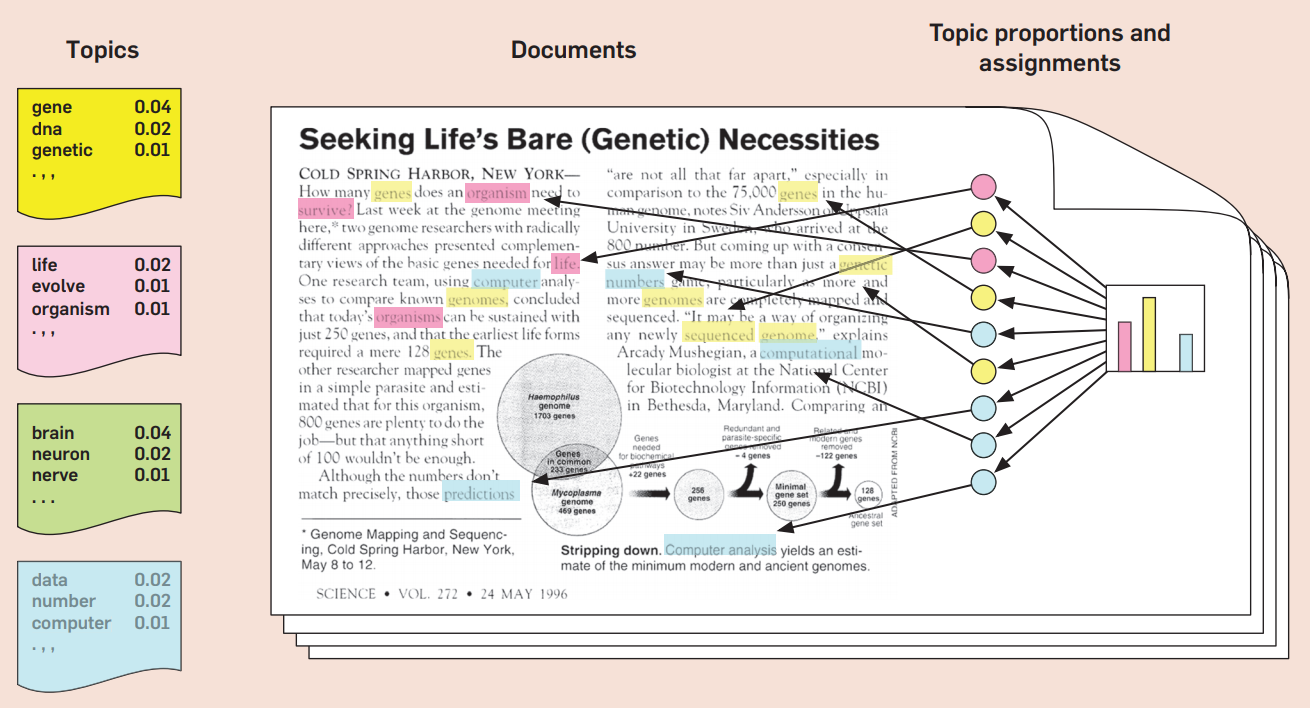
\includegraphics[width=0.8\textwidth]{document/images/lda_topic_model.png}
    % Der Teil in eckigen Klammern ist der Kurztitel für das Table of Contents
    \caption[Schematische Darstellung eines LDA Topic Modelings]{Schematische Darstellung eines LDA Topic Modelings. Quelle: \citetitle{blei_2012} \parencite{blei_2012}}
    \label{fig:lda_example}
\end{figure}

% Wenn wir nicht wollen, dass ein Kapitel auf einer neuen Seite startet, nutzen wir folgenden Befehl hier:
{\let\clearpage\relax \chapter{Theoriefindung}}



%% Bibliography

\setstretch{1.0}
\printbibliography[title={Literaturverzeichnis}]

\end{document}